\documentclass[report,12pt,openright,oneside,a4paper,brazil]{abntex2}
\usepackage[utf8]{inputenc}
\usepackage{graphicx}
\usepackage{subfig}
\usepackage{lmodern}
\usepackage{float}
\usepackage[brazil]{babel}
\usepackage{booktabs}
\usepackage{longtable}
\usepackage{setspace}
\usepackage{parskip}
\usepackage{leading}
\usepackage{amsmath,esint}
\usepackage{amssymb}
\usepackage{physics}
\usepackage{indentfirst}
\usepackage[newfloat]{minted}

%Configuring the code environment
\newminted{python}{frame=lines,framerule=2pt}
\newenvironment{code}{\captionsetup{type=listing}}{}
\SetupFloatingEnvironment{listing}{name=Código}

\renewcommand{\ABNTEXchapterfont}{\fontfamily{cmr}\fontseries{b}\selectfont}
%%\renewcommand{\ABNTEXchapterfontsize}{\LARGE}

\titulo{Título}
\autor{
    \makebox[.6\textwidth]{
    	Guilherme Fortes Evangelista \hfill 
        RA:	21062515}\\
	\makebox[.6\textwidth]{
    	Henrique Dias Gomes \hfill
        RA: 11046715}\\
	\makebox[.6\textwidth]{
    	Júlio César Lopes Ducini de Carvalho\hfill 
        RA: 11023516}\\
	\makebox[.6\textwidth]{
    	Matheus Ianello \hfill 
        RA: 11032115}
    \makebox[.6\textwidth]{
    	Rodrigo Tardini Paulino\hfill 
        RA: 11006916}}
\instituicao{Universidade Federal do ABC}
\local{Santo André}
\tipotrabalho{Relatório}
\orientador{Breno Marques Gonçalves Teixeira\\}
\date{Março de 2019}

\renewcommand{\imprimircapa}{%
\begin{capa}%
	\begin{figure}[ht]
		\centering
		
\includegraphics[scale=0.6]{logo.jpg}
		\label{fig:logo}
	\end{figure}
	\begin{center}
		\textbf{\large Óptica - NHT3044-15}
		\vfill
    	{\LARGE\textbf{\imprimirtitulo}}
    	\vfill
    	Docente: \imprimirorientador
    	\vspace*{1cm}
		\imprimirautor
		\vfill
    	\imprimirlocal \\
    	\imprimirdata
	\end{center}
\end{capa}
}

\setlength{\parindent}{1.3cm}
\setlength{\parskip}{0.2cm}

\begin{document}
\imprimircapa

\pagenumbering{arabic}

\chapter{Parte I}

\begin{table}[H]
\centering
\caption{My caption}
\label{my-label2}
\begin{tabular}{|c|c|c|c|c|}
\hline
$u$ (cm) & $u^{-1}$ (m$^{-1}$) & $v$ (cm) & $v^{-1}$ (m$^{-1}$) & $M_{(u/v)}$ \\ \hline
29,00  &  $3,448 \pm 0,001$  &  16,00  &  $6,250 \pm 0,002$  &  $1,8125 \pm 0,0007$  \\ \hline
24,75  &  $4,040 \pm 0,001$  &  17,75  &  $5,634 \pm 0,002$  &  $1,3944 \pm 0,0005$  \\ \hline
20,90  &  $4,785 \pm 0,001$  &  19,50  &  $5,128 \pm 0,001$  &  $1,0718 \pm 0,0004$  \\ \hline
19,55  &  $5,115 \pm 0,001$  &  21,25  &  $4,706 \pm 0,001$  &  $0,9200 \pm 0,0003$  \\ \hline
17,60  &  $5,682 \pm 0,002$  &  23,00  &  $4,348 \pm 0,001$  &  $0,7652 \pm 0,0003$  \\ \hline
16,95  &  $5,900 \pm 0,002$  &  24,75  &  $4,040 \pm 0,001$  &  $0,6848 \pm 0,0002$  \\ \hline
16,40  &  $6,098 \pm 0,002$  &  26,50  &  $3,774 \pm 0,001$  &  $0,6189 \pm 0,0002$  \\ \hline
15,75  &  $6,349 \pm 0,002$  &  28,25  &  $3,540 \pm 0,001$  &  $0,5575 \pm 0,0002$  \\ \hline
\end{tabular}
\end{table}

\begin{table}[H]
\centering
\caption{My caption}
\label{my-label}
\begin{tabular}{|c|c|}
\hline
$h'$ (cm) & $M_{(h'/h)}$ \\ \hline
1,9  & $1,9 \pm 0,1$  \\ \hline
1,4  & $1,4 \pm 0,1$  \\ \hline
1,1  & $1,1 \pm 0,1$  \\ \hline
0,9  & $0,9 \pm 0,1$  \\ \hline
0,7  & $0,7 \pm 0,1$  \\ \hline
0,6  & $0,6 \pm 0,1$  \\ \hline
0,6  & $0,6 \pm 0,1$  \\ \hline
0,6  & $0,6 \pm 0,1$  \\ \hline
\end{tabular}
\end{table}

\begin{figure}[H]
    \centering
    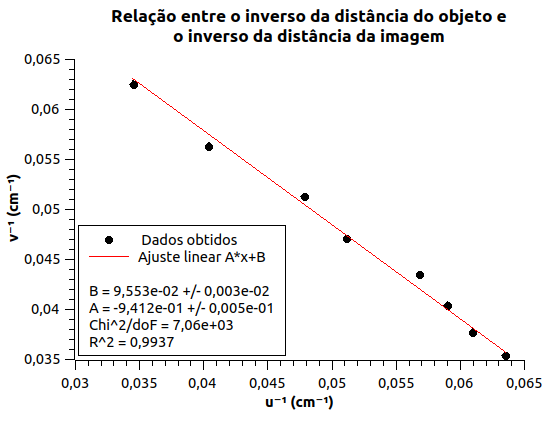
\includegraphics[scale=0.7]{Figuras/distObjIm.png}
    \caption{Caption}
    \label{fig:my_label}
\end{figure}

\begin{figure}[H]
    \centering
    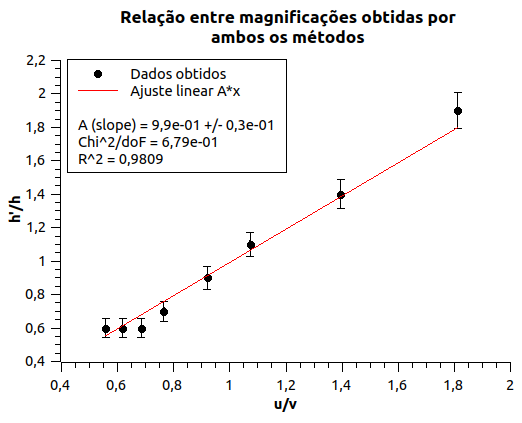
\includegraphics[scale=0.7]{Figuras/magni.png}
    \caption{Caption}
    \label{fig:my_label2}
\end{figure}

\chapter{Parte II}

\chapter{Parte III}

\newpage
\appendix

\newpage

\addcontentsline{toc}{chapter}{\bibname}
\bibliographystyle{abntex2-num}
\bibliography{refs.bib}
\nocite{*}

\chapter{Demonstrações}

\chapter{Propagação de incertezas}

\end{document}